\originalchapter{8.323 作业6题解}
本章据 MIT OCW 8.323(2023 春)\href{https://ocw.mit.edu/courses/8-323-relativistic-quantum-field-theory-i-spring-2023/mit8_323_s23_pset06.pdf}{作业6}及\href{https://ocw.mit.edu/courses/8-323-relativistic-quantum-field-theory-i-spring-2023/mit8_323_s23_pset_06sol.pdf}{官方解}中文重编,补充图的计数与核查,不是官方中文版.沿用 $(+---)$.令
\[
D(x)=\bra0T\phi(x)\phi(0)\ket0=\int\frac{\dd^4p}{(2\pi)^4}\e^{-\ii p\cdot x}d(p),\qquad d(p)=\frac{\ii}{p^2-m^2+\ii0}.
\]
本套“连通”严格指图只有一个连通分量;“不含真空泡”允许若干各含外线的分量,二者不能混同.路径积分的场在 $t\to\pm\infty$ 及 $|\mathbf x|\to\infty$ 消失,并以 $\ii0$ 规定真空投影.微扰关联函数为
\[
G_n=\frac{\bra0T\phi(x_1)\cdots\phi(x_n)\exp[-\ii\int_{-\infty}^{\infty}H_I(t)\dd t]\ket0}
{\bra0T\exp[-\ii\int_{-\infty}^{\infty}H_I(t)\dd t]\ket0},\qquad
H_I=\frac{\lambda}{4!}\int\dd^3x\,\phi^4.
\]
时间序作用于展开后所有场,包括积分内的 $H_I(t_j)$;例如第 $r$ 项是 $(-\ii)^r/r!\int\prod_j\dd t_j\,T[H_I(t_1)\cdots H_I(t_r)]$.以下积分保留为带同一调节的形式表达,未宣称发散环积分已经有限.

\originalsection{原题1}
\begin{exercise}
继续作业4原题2.定义 $Z[J]=\int\mathcal D\phi\,\e^{\ii\int\dd^4x(\Lag_0+J\phi)}$、$Z_0=Z[0]$.接受适当 $\ii0$ 下 $\bra{0,+\infty}0,-\infty\rangle=Z[J]/Z_0$,不必推导此等式.直接计算高斯路径积分,求 $P_0=|Z[J]/Z_0|^2$,并核对作业4原题2(h).
\end{exercise}
\begin{solution}
分部积分后二次核是 $A=-(\Box+m^2)+\ii0$,动量表示为 $A(p)=p^2-m^2+\ii0$.平移积分变量 $\phi\mapsto\phi-A^{-1}J$,高斯行列式与无源分母相消,得
\[
\frac{Z[J]}{Z_0}=\exp\left[-\frac{\ii}{2}\int\frac{\dd^4p}{(2\pi)^4}\frac{J(p)J(-p)}{p^2-m^2+\ii0}\right].
\]
源为实函数,$J(p)J(-p)=|J(p)|^2$.用 $1/(a+\ii0)=\operatorname{PV}(1/a)-\ii\pi\delta(a)$,指数实部是 $-\tfrac\pi2\int\dd^4p\,|J(p)|^2\delta(p^2-m^2)/(2\pi)^4$.因此
\[
\log P_0=-\pi\int\frac{\dd^4p}{(2\pi)^4}|J(p)|^2\delta(p^2-m^2).
\]
$p^0$ 积分产生正负两个壳,各有 $1/(2\omega_p)$.负壳令 $\mathbf p\mapsto-\mathbf p$,利用实源关系变成正壳,两个壳抵消 $\pi/(2\pi)$ 的 $1/2$,所以 $\log P_0=-\intp|J(\omega_p,\mathbf p)|^2/(2\omega_p)=-\lambda$.主值部分只产生相位;$P_0=\e^{-\lambda}$ 与算符方法一致.
\end{solution}

\originalsection{原题2}
\begin{exercise}
(a) 列出 $\bra0T\phi(x_1)\phi(x_2)\exp[-\ii\int H_I\dd t]\ket0$ 到 $\order(\lambda^2)$ 的全部连通图及各自对称因子.在 $\lambda^0,\lambda^1$ 阶写出坐标、动量空间表达式;$\lambda^2$ 阶任选一图写出两种表达式.
(b) 列出 $G_4(x_1,x_2,x_3,x_4)$ 到 $\order(\lambda^2)$ 的全部连通图,任选两图写出坐标与动量表达式.不要求计算环积分.
\end{exercise}
\begin{solution}
每个四价顶点带 $-\ii\lambda$,对称因子 $S$ 的约定是图贡献乘 $1/S$.外点带固定标签,交换不同外点不是图的内部对称.下列图中实心点是积分顶点,细线端点是外点;自环是同点收缩.

(a) 二点函数共有五种图:自由线一张,一阶单自环一张,二阶三张.二阶代表图依次如下:
\begin{center}
\begin{tikzpicture}[scale=.85,every node/.style={font=\small}]
\node (x) at (0,0) {$x_1$};\node[circle,fill,inner sep=2pt,label=below:$z$] (z) at (1,0) {};\node[circle,fill,inner sep=2pt,label=below:$w$] (w) at (3,0) {};\node (y) at (4,0) {$x_2$};
\draw (x)--(z)--(w)--(y);\draw (z) to[out=65,in=115,looseness=8] (z);\draw (w) to[out=65,in=115,looseness=8] (w);
\node at (2,-.8) {串联双自环,$S=4$};
\begin{scope}[xshift=5.6cm]
\node (x) at (0,.6) {$x_1$};\node (y) at (0,-.6) {$x_2$};\node[circle,fill,inner sep=2pt,label=below:$z$] (z) at (1,0) {};\node[circle,fill,inner sep=2pt,label=below:$w$] (w) at (3,0) {};
\draw (x)--(z)--(y);\draw (z) to[bend left=22] (w);\draw (z) to[bend right=22] (w);\draw (w) to[out=65,in=115,looseness=8] (w);\node at (1.8,-.8) {自环插入,$S=4$};
\end{scope}
\begin{scope}[yshift=-2.4cm,xshift=2.8cm]
\node (x) at (0,0) {$x_1$};\node[circle,fill,inner sep=2pt,label=below:$z$] (z) at (1,0) {};\node[circle,fill,inner sep=2pt,label=below:$w$] (w) at (3,0) {};\node (y) at (4,0) {$x_2$};\draw (x)--(z);\draw (w)--(y);\draw (z)--(w);\draw (z) to[bend left=30] (w);\draw (z) to[bend right=30] (w);\node at (2,-.8) {三线日落图,$S=6$};
\end{scope}
\end{tikzpicture}
\end{center}
完整表达式也可直接编码图的每条边:
\begin{align*}
C_0&=D(x_1-x_2),&&S=1,\\
C_1&=\frac{-\ii\lambda}{2}\int\dd^4z\,D(x_1-z)D(x_2-z)D(0),&&S=2,\\
C_{2a}&=\frac{(-\ii\lambda)^2}{4}\int\dd^4z\dd^4w\,D(x_1-z)D(z-w)D(w-x_2)D(0)^2,&&S=4,\\
C_{2b}&=\frac{(-\ii\lambda)^2}{4}\int\dd^4z\dd^4w\,D(x_1-z)D(x_2-z)D(z-w)^2D(0),&&S=4,\\
C_{2c}&=\frac{(-\ii\lambda)^2}{6}\int\dd^4z\dd^4w\,D(x_1-z)D(x_2-w)D(z-w)^3,&&S=6.
\end{align*}
这里两条外线在自环插入图中必须接同一个顶点,才使两个顶点都四价.原官方解表格的一处坐标式未保持这个接法,本章已按图的四价性校正.
为核查全部性,若两个顶点各接一条外线,设它们之间有 $r$ 条边,则 $r+2\ell_z=r+2\ell_w=3$,故 $r=1$ 或3,分别给出 $C_{2a},C_{2c}$.若两条外线接同一个顶点,则 $r+2\ell_z=2,r+2\ell_w=4$,连通要求 $r>0$,唯一解 $r=2,\ell_z=0,\ell_w=1$,就是 $C_{2b}$.
因子可从 $1/[2!(4!)^2]$ 与 Wick 配对数核对:$C_{2a}$ 有 $2\times4\times4\times3\times3=288$ 种配对;$C_{2b}$ 有 $2\times(4\times3)\times\binom42\times2!=288$ 种;$C_{2c}$ 有 $2\times4\times4\times3!=192$ 种,分别除以1152得到 $1/4,1/4,1/6$.一阶则 $4\times3/4!=1/2$.
取二点动量 $p$ 流入、$p'$ 流出,傅里叶核为 $\e^{\ii p\cdot x_1-\ii p'\cdot x_2}$.令 $I=\int\dd^4q\,d(q)/(2\pi)^4$,则
\begin{align*}
\widetilde C_0&=(2\pi)^4\delta^{(4)}(p-p')d(p),\\
\widetilde C_1&=(2\pi)^4\delta^{(4)}(p-p')\frac{-\ii\lambda}{2}d(p)^2I,\\
\widetilde C_{2c}&=(2\pi)^4\delta^{(4)}(p-p')\frac{(-\ii\lambda)^2}{6}d(p)^2
\int\frac{\dd^4q\dd^4r}{(2\pi)^8}d(q)d(r)d(p-q-r).
\end{align*}
最后一行选了日落图,其两独立环动量及第三线动量均已写明.

(b) 零阶不存在四外点的连通图.一阶有一个四外线顶点,$S=1$.二阶有四张外腿自环插入图(插入外腿 $a=1,2,3,4$,各 $S=2$),以及 $s,t,u$ 三张双线泡图(外点分组 $12|34,13|24,14|23$,各 $S=2$).以下画一阶、第一条外腿插入和 $s$ 道代表;其余通过所列标签置换得到.
\begin{center}
\begin{tikzpicture}[scale=.7,every node/.style={font=\small}]
\node[circle,fill,inner sep=2pt] (z) at (1,0) {};\node (a) at (0,1) {$1$};\node (b) at (0,-1) {$2$};\node (c) at (2,1) {$3$};\node (d) at (2,-1) {$4$};\draw (a)--(z)--(b);\draw (c)--(z)--(d);\node at (1,-1.6) {一阶};
\begin{scope}[xshift=4cm]
\node[circle,fill,inner sep=2pt] (z) at (1,0) {};\node[circle,fill,inner sep=2pt] (w) at (3,0) {};\node (a) at (0,0) {$1$};\node (b) at (4,1) {$2$};\node (c) at (4,0) {$3$};\node (d) at (4,-1) {$4$};\draw (a)--(z)--(w);\draw (w)--(b);\draw (w)--(c);\draw (w)--(d);\draw (z) to[out=65,in=115,looseness=8] (z);\node at (2,-1.6) {外腿1插入};
\end{scope}
\begin{scope}[xshift=10cm]
\node[circle,fill,inner sep=2pt] (z) at (1,0) {};\node[circle,fill,inner sep=2pt] (w) at (3,0) {};\node (a) at (0,1) {$1$};\node (b) at (0,-1) {$2$};\node (c) at (4,1) {$3$};\node (d) at (4,-1) {$4$};\draw (a)--(z)--(b);\draw (c)--(w)--(d);\draw (z) to[bend left=25] (w);\draw (z) to[bend right=25] (w);\node at (2,-1.6) {$12|34$ 泡图};
\end{scope}
\end{tikzpicture}
\end{center}
全部性也可由顶点度数得出:外腿分配只能为 $1+3$ 或 $2+2$.前者强制一条内部连线和一个自环,后者强制两条内部连线;$0+4$ 无法连通.外腿插入的自环翻转给 $S=2$,泡图两条内部线交换给 $S=2$.
任选的一阶图及 $12|34$ 泡图的两种表达为
\begin{align*}
G_{4,\mathrm{tree}}&=(-\ii\lambda)\int\dd^4z\,\prod_{a=1}^4D(x_a-z),\\
G_{4,s}&=\frac{(-\ii\lambda)^2}{2}\int\dd^4z\dd^4w\,D(x_1-z)D(x_2-z)D(z-w)^2D(x_3-w)D(x_4-w),\\
\widetilde G_{4,\mathrm{tree}}&=(-\ii\lambda)(2\pi)^4\delta^{(4)}(\textstyle\sum_a p_a)\prod_a d(p_a),\\
\widetilde G_{4,s}&=\frac{(-\ii\lambda)^2}{2}(2\pi)^4\delta^{(4)}(\textstyle\sum_a p_a)\prod_a d(p_a)
\int\frac{\dd^4q}{(2\pi)^4}d(q)d(p_1+p_2-q).
\end{align*}
这里所有四个动量流入.为了使插入图也能复算,其坐标式为
$\frac{(-\ii\lambda)^2}{2}\int\dd^4z\dd^4w\,D(x_a-z)D(0)D(z-w)\prod_{b\ne a}D(x_b-w)$,动量式是在共同因子 $(2\pi)^4\delta^{(4)}(\sum p)\prod_bd(p_b)$ 上再乘 $(-\ii\lambda)^2d(p_a)I/2$.
\end{solution}

\originalsection{原题3}
\begin{exercise}
自由真空归一为1,设 $Z_0=\bra0T\exp[-\ii\int H_I\dd t]\ket0$、$W_0=\log Z_0$.
(a) 证明长时间真空振幅中 $W_0=C-\ii\varepsilon VT$,$\varepsilon$ 是相互作用理论与自由理论真空能量密度之差,$T=t-t_0$,原题称 $C$ 为与时空体积无关的常数;(b) 证明 $W_0$ 是所有连通真空图之和,论证应能推广到一般理论;(c) 写出 $\varepsilon$ 到 $\order(\lambda^2)$ 的表达式,可以只写传播子的坐标或动量积分,不必计算,且须承认发散.
\end{exercise}
\begin{solution}
(a) 先放入体积 $V$ 的盒子.在相互作用绘景,
\[
Z_0(T)=\e^{\ii E_0T}\bra0\e^{-\ii HT}\ket0
=\e^{\ii E_0T}\sum_n|\braket{n}{0}|^2\e^{-\ii E_nT}.
\]
适当的负虚时间分量使激发态相对最低态衰减;长时间真空投影给
$Z_0\sim|\braket{\Omega}{0}|^2\e^{-\ii(E_\Omega-E_0)T}$,所以
$W_0\sim\log|\braket{\Omega}{0}|^2-\ii\varepsilon VT$、$\varepsilon=(E_\Omega-E_0)/V$.
须区分两种常数含义:固定盒子时重叠项独立于 $T$,但一般可依赖 $V$;仅凭题设不能证明它严格独立于空间体积.采用归一化的绝热真空边界态,或把边界重叠剔除来定义体积项,则可令 $C=0$,得到原题所用“与时空体积无关”的形式.能量密度由 $VT$ 的系数抽取,不受这个边界归一选择影响;也不需要官方解中的“小能量差”近似.
(b) 记每种连通真空图的完整积分连同其内部对称因子为 $v_i$.一般真空图唯一分解为 $n_i$ 份第 $i$ 类连通图.独立顶点积分使其贡献相乘,同类分量交换额外给 $1/n_i!$,因此形式级数为
\[
Z_0=\sum_{\{n_i\}}\prod_i\frac{v_i^{n_i}}{n_i!}
=\prod_i\sum_{n_i=0}^\infty\frac{v_i^{n_i}}{n_i!}
=\exp\left(\sum_i v_i\right).
\]
空图贡献1.取满足 $W_0(\lambda=0)=0$ 的对数分支,得到 $W_0=\sum_i v_i$.这是关于形式微扰级数的组合恒等式,不依赖级数收敛,也不依赖相互作用一定是四次.
(c) 一阶连通真空图是单顶点两个自环,配对数3,因子 $3/4!=1/8$.二阶有两种:每个顶点各一个自环、两顶点间两条线,$S=16$;两顶点间四条线,$S=48$.前者配对数 $\binom42^2 2!=72$,后者配对数 $4!=24$,除以 $2!(4!)^2=1152$ 即核对 $1/16,1/48$.
\begin{center}
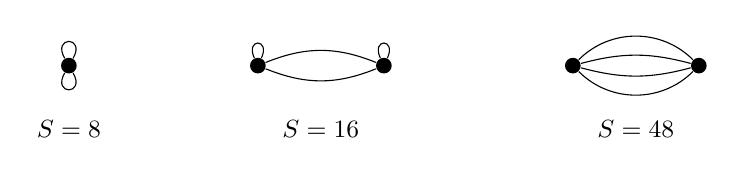
\begin{tikzpicture}[scale=.8,every node/.style={font=\small}]
\node[circle,fill,inner sep=2pt] (z) at (1,0) {};\draw (z) to[out=60,in=120,looseness=8] (z);\draw (z) to[out=240,in=300,looseness=8] (z);\node at (1,-1) {$S=8$};
\begin{scope}[xshift=3cm]
\node[circle,fill,inner sep=2pt] (z) at (1,0) {};\node[circle,fill,inner sep=2pt] (w) at (3,0) {};\draw (z) to[out=65,in=115,looseness=8] (z);\draw (w) to[out=65,in=115,looseness=8] (w);\draw (z) to[bend left=22] (w);\draw (z) to[bend right=22] (w);\node at (2,-1) {$S=16$};
\end{scope}
\begin{scope}[xshift=8cm]
\node[circle,fill,inner sep=2pt] (z) at (1,0) {};\node[circle,fill,inner sep=2pt] (w) at (3,0) {};\draw (z) to[bend left=45] (w);\draw (z) to[bend left=15] (w);\draw (z) to[bend right=15] (w);\draw (z) to[bend right=45] (w);\node at (2,-1) {$S=48$};
\end{scope}
\end{tikzpicture}
\end{center}
积分中的整体平移坐标给 $VT$,其余为相对坐标,故
\[
\frac{W_0}{VT}=\frac{-\ii\lambda}{8}D(0)^2
+\frac{(-\ii\lambda)^2}{16}D(0)^2\int\dd^4z\,D(z)^2
+\frac{(-\ii\lambda)^2}{48}\int\dd^4z\,D(z)^4+\order(\lambda^3).
\]
由 $\varepsilon=\ii W_0/(VT)$ 抽取体积系数,
\[
\varepsilon=\frac\lambda8D(0)^2-\frac{\ii\lambda^2}{16}D(0)^2\int\dd^4z\,D(z)^2
-\frac{\ii\lambda^2}{48}\int\dd^4z\,D(z)^4+\order(\lambda^3).
\]
上述同点传播子和环积分需调节及重整化;本题只要求写出未经求值的微扰结构.
\end{solution}

\originalsection{原题4}
\begin{exercise}
证明任意 $n$ 点关联函数的分子、分母相除后,所有带真空图因子的图都消去,只留下不含真空图因子的图.一般 $H_I$ 下也成立,但证明四次相互作用已足够.不应将这一结论误写为“只剩完全连通图”.
\end{exercise}
\begin{solution}
每个带外点的 Wick 图都有唯一分解:保留所有含至少一个外点的连通分量,组成图 $D_\alpha$;把其余无外点分量作为真空图.$D_\alpha$ 的外点带固定标签,不能和无外点真空分量交换.因此其内部对称因子与真空图因子相互独立.
设 $D_\alpha$ 已包括其 Wick 系数.对固定 $D_\alpha$ 附加任意数目的各类真空分量,原题3的计数给出
$D_\alpha\prod_i\sum_{n_i\ge0}v_i^{n_i}/n_i!=D_\alpha\e^{\sum_i v_i}=D_\alpha Z_0$.再遍历所有不含真空分量的图,分子为 $Z_0\sum_\alpha D_\alpha$;分母正是 $Z_0$,故 $G_n=\sum_\alpha D_\alpha$.由于 $Z_0$ 常数项是1,形式级数除法是合法的.
例如自由四点函数的三种 $D(x_i-x_j)D(x_k-x_l)$ 仍然留下:每条线都含外点,没有真空泡,但整图不连通.若要提取完全连通的关联函数,还须对带源生成泛函取对数;真空泡消去本身并不做这一步.
\end{solution}
